\chapter{Portable Executable Format} \label{chap:peformat}

The \PE{} is a file format for image files used by Microsoft products for 32- and 64-bit system architectures. It is the successor of the \NZ{} file format for 16-bit systems. The \PE{} format is described in the \PECOFF{} \cite{pespec}

\PE{} file types, which are relevant for this thesis, are \DLL{} and \EXE{} files. \DLL{} files export functions or data other programs can use. They can have various file endings, including \emph{.sys}, \emph{.dll}, \emph{ocx}, \emph{.cpl} and \emph{.drv}. (\cf{} \cite{micrdll}) A \DLL{} usually has no main entry point, but is loaded into the context of another process.
\EXE{} files have the file ending \emph{.exe}. They usually don't export any functions. The system creates a new process upon launching the \EXE{}.
The system recognizes the file type by a certain flag in the \PE{} headers. (see \ref{dllflag})

Both, \EXE{} and \DLL{} files, are considered as \emph{image files} by the \PECOFF{}, because they contain executable code. \todo{Beleg} In contrast to image files are object files (Common Object File Format or {COFF}), which don't contain executable code. The Common Object File Format is not an issue in the thesis.

\portex{} extracts the information from the \PE{} format to assist in analysing malware. Therefore knowledge about the \PE{} format is neccessary to understand the inner workings of the library \portex{}.

\section{General Structure and PE Headers}

\begin{figure}
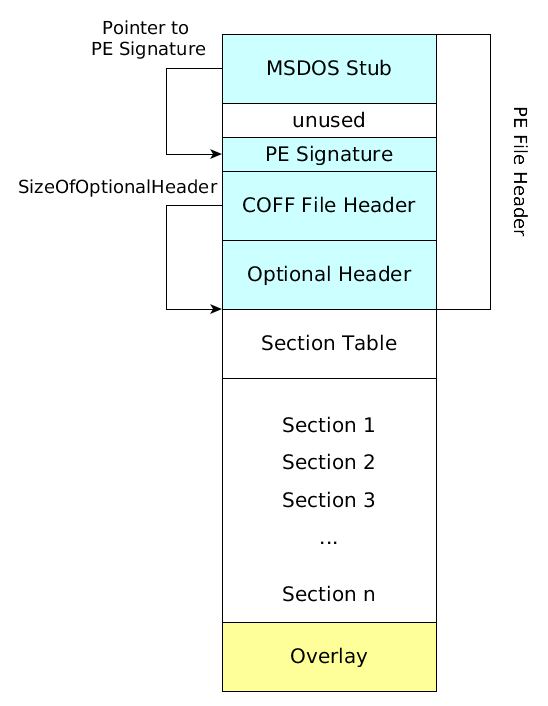
\includegraphics[width=.98\textwidth, height=\textheight,keepaspectratio]{graphics/peformat}
\caption{Structure of a PE file}
\label{fig:peformat} 
\end{figure}

Figure~\ref{fig:peformat} illustrates the structure of a \PE{} file. An executable \PE{} file always starts with the MS-DOS Stub. This is an application which is able to run in MS-DOS. The standard MS-DOS stub prints the message \enquote{This program cannot be run in DOS mode} and closes right after. 

To determine if a file is of a certain file format, signatures are used. The file format signature is usually at the very beginning of the file. Since the \PE{} starts with the MS-DOS stub, which has a file signature itself, the \PE{} signature is placed after. \todo{MZ, PE00} The offset to the \PE{} signature is defined in location 0x3c of the MS-DOS stub, thus enables Windows to properly execute the \PE{} file. 

Right after the signature follow the COFF File Header, the Optional Header and the Section Table. The COFF File Header contains information about the type of the target machine, the number of sections, a time date stamp that indicates when the file was created, the size of the Optional Header.and flags that indicate file characteristics including a flag that indicates whether the file is a \DLL{}\label{dllflag}.

Despite its name the Optional Header is mandatory for image files. Only object files don't need it. The Optional Header has three parts: Standard Fields, Windows Specific Fields and a Data Directory Table.
The Standard Fields of the Optional Header contain information necessary for loading and running the file. They determine for example, whether the image file allows a 64-bit address space (PE32+) or is limited to a 32-bit address space (PE32). They also declare \ia{} the size of initialized, uninitialized data, the size of the code, the linker versions and the entry point of the image file.
The Windows Specific fields provide additional information for the Windows loader and linker like the operating systems the image file can run on, alignment values, dll characteristics and the number of data directories in the Data Directory Table.
A Data Directory Table entry consists of address and size for a table or string that the system uses. Examples are the import table, the export table or the resource table. \todo{references}

The Section Table consists of the section headers for the sections that make up the rest of the \PE{} file. A section header describes \ia{} characteristics, size, name and location of a section.

While the PE Headers described above are located at a fixed file offset, the rest of the PE contains data defined by pointers in the PE Headers. Data that was appended to the file, but is not part of the \PE format is called \emph{overlay}. Overlay is not mapped into memory. The overlay is used by some applications as an easy way to store arbitrary data.

\section{Special Sections}

Sections may contain arbitrary information, which is only relevant to the application using them; but some sections have a special meaning. Their format is described in the \PECOFF{} \cite{pespec}. These sections are recognized by entries in the Data Directory Table of the Optional Header or certain flags in the Section Table. They have typical section names which are also used in the specification to refer to the sections. These names are not mandatory, but a convention. That's why they can not be relied on while trying to find certain sections.
Some of these special sections are described right after. \todo{sections that are recognized by portex}

\subsection*{Import Section}

\begin{figure}
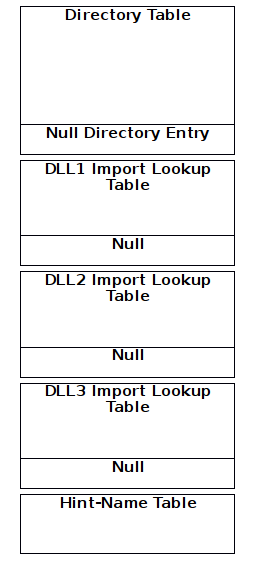
\includegraphics[width=.98\textwidth, height=\textheight,keepaspectratio]{graphics/importsection}
\caption{Typical Import Section Layout by \protect{\cite[\p{61}]{pespec}}}
\label{fig:import} 
\end{figure}

Every image file that imports symbols has an \emph{Import Section}, also called \emph{.idata Section}.
The Import Section contains the Import Directory Table, several Import Lookup Tables, the Hint-Name Table and the \IAT{}. A typical layout of the Import Section is in figure~\ref{fig:import}

Every Import Directory Table entry points to an Import Lookup Table. Each Import Lookup Table describes the imported symbols of a single \DLL{}.

The Hint-Name table entries have a hint and an ASCII name of the import. Each hint is an index to the Export Name Pointer Table of the \DLL{} the image is importing from. Hints speed up the lookup of imports.

Null entries mark the end of the Import Directory Table and the Import Lookup Table.

The \IAT{} is identical to the Import Directory Table except while the image is bound. In the latter case the \IAT{} entries are overwritten with memory addresses of the imported symbols.

\subsection*{Export Section}

The \emph{.edata Section} or \emph{Export Section} is generally found in \useacronym[s]{DLL}. The section begins with the Export Directory Table, which contains general information and addresses to resolve imports from this section. The Export Directory Table points to an array of addresses called Export Address Table. Each address either points to code or data within the current image file, or is a forwarder address which points to a symbol in another \DLL{}. 

Other image files have two ways to import symbols from the current image file: They either use an index into the Export Address Table (the index is also called \emph{ordinal}) or they use a public name of the symbol. Ordinals are defined in the Ordinal Table; public names are defined in the Export Name Table.

Entries of the Ordinal Table correspond to the Export Name Pointer Table entries by their position. Every entry is an ordinal that represents an index in the Export Address Table.

The Export Name Pointer Table is an array of addresses which point to names of the Export Name Table. These names are null-terminated ASCII strings. They are the public names that other image files can use to import the symbols.

Listing~\ref{lst:exportsample} shows example contents for a \DLL{} with two exported symbols: \texttt{DLL2Print} and \texttt{DLL2ReturnJ}.

\lstinputlisting[caption=Example for Export Section contents,captionpos=t,label=lst:exportsample]{listings/edata_sample}

\subsection*{Resource Section}

Resources of a \PE{} can be \ia{} icons, text, windows, copyright information. They are saved as an entry in the \emph{Resource Section}, which also has the name \emph{.rsrc Section}. The Resource Section is build up as a tree with the actual resource addresses as leaves. While \(2^{31}\) levels can be used according to the \PECOFF{} \cite[\p{100}]{pespec}, Windows only uses three levels with the first level node being the type, the second being the name and the third being the language information. Figure~\ref{fig:resourcetree} illustrates the structure of a resource tree.

\begin{figure}
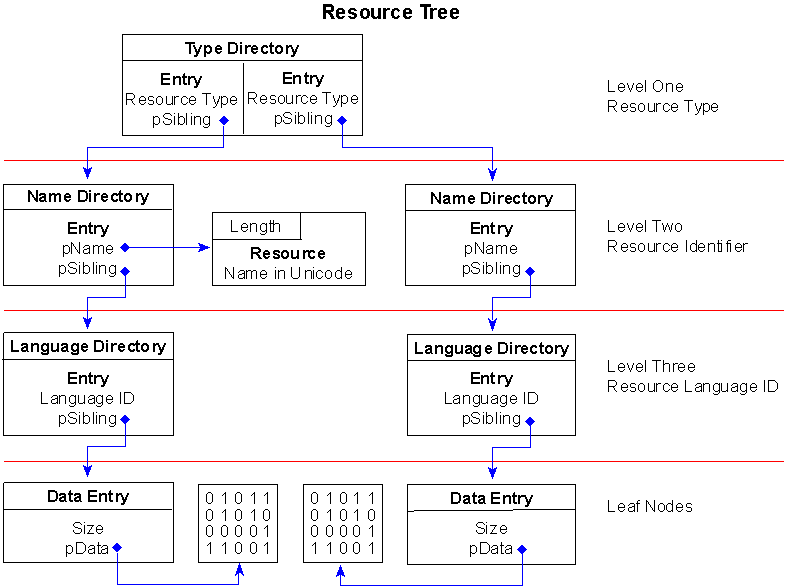
\includegraphics[width=.98\textwidth, height=\textheight,keepaspectratio]{graphics/resourcetree}
\caption{ Resource tree structure by \protect{\cite{kath13}}}
\label{fig:resourcetree} 
\end{figure}

\subsection*{Debug Section and Debug Directory}

Whereas most sections can be at an arbitrary location in the file, the \emph{Debug Section} (aka \emph{.debug Section}) must be placed as the very end of the image file. The reason is that the loader doesn't map this section into memory. Image files contain per default of the linker only a Debug Directory (as pointed to by the Data Directory Table), but not a Debug Section (see \cite[\p{78}]{pespec}). Thus the Debug Directory is either located in the Debug Section if it exists, in any other section of the \PE{} or not in any section at all.

Every Debug Directory entry defines \ia{} size, location and the type (format) of a debug information block. 



